\documentclass{article}

\usepackage{amssymb}
\usepackage{caption}
\usepackage{color}
\usepackage{colortbl}
\usepackage{enumitem}
\usepackage[T1]{fontenc}
\usepackage{hyperref}
\usepackage{minted}
\usepackage{tcolorbox}
\usepackage{tikz}
\usepackage{xcolor}

\hypersetup
{
    colorlinks=true,
    linkcolor=blue,
    filecolor=magenta,
    urlcolor=cyan
}

\newcommand{\crnotice}[1]
{
    \begin{center}
        \colorbox{red!15}{\parbox{\textwidth}{#1}}
    \end{center}
}
\newcommand{\sekcija}[1]{\section{\textsc{#1}}}
\newcommand{\dio}[1]{\sekcija{#1. dio}}
\newcommand{\zadatak}[1]{\subsection{Zadatak #1}}
\newcommand{\odgovor}{\subsubsection*{Odgovor}}
\newcommand{\code}[1]{\colorbox{blue!11}{\texttt{#1}}}

\renewcommand{\contentsname}{\textsc{Sadržaj}}

\setcounter{secnumdepth}{0}

\newminted[ccode]{text}{fontsize=\small, tabsize=4, breaklines}

\begin{document}
\begin{titlepage}
    \centering
    \vspace*{\fill}

    \huge
    \textbf{\textsc{Formalne metode u oblikovanju sustava}} \\
    
    \vspace*{0.5cm}
    
    \large
    \textsc{3. domaća zadaća - ProMeLa i Spin} \\

    \vspace*{\fill}
    \textsc{Zagreb, svibanj 2020.}
\end{titlepage}

\tableofcontents
\pagebreak



\sekcija{Izjava}

Zadaci priloženi uz ovu domaću zadaću pripadaju njihovim vlasnicima te služe isključivo u edukacijske svrhe. Bilo koja promjena originala je isključivo radi estetske i funkcionalne prirode i ne mijenja smisao informacije. Također, takve promjene ne primijenjuje nikakvu drukčiju licencu niti se smatraju intelektualnim vlasništvom uređivača.
\newline

Uz ovu datoteku obično dolaze i primjerci kôda, koji su zaštićeni licencom:

\crnotice
{
    Copyright 2020 Miljenko Šuflaj
    \newline

    Licensed under the Apache License, Version 2.0 (the "License");
    you may not use this file except in compliance with the License.
    You may obtain a copy of the License at
    \newline

        \quad
        http://www.apache.org/licenses/LICENSE-2.0
        \newline

    Unless required by applicable law or agreed to in writing, software
    distributed under the License is distributed on an "AS IS" BASIS,
    WITHOUT WARRANTIES OR CONDITIONS OF ANY KIND, either express or implied.
    See the License for the specific language governing permissions and
    limitations under the License.
}

\sekcija{Napomena}

Iako u uputama piše da se koriste \texttt{.prm} datoteke, često će se odgovarati s \texttt{.pml} datotekama. Ovo vas ne bi trebalo zbuniti, jer su datoteke sadržajem iste, a ekstenzija je drukčija samo zato što je uz nju u Visual Studio Code-u dostupno bojanje teksta, pa je lakše pisati taj kod. Isto tako, kad god u odgovoru piše da se pokreće neki kod, to se vrši u korijenskom direktoriju zadaće (tj. u DZ3).

\pagebreak





\dio{1}

Zadana su dva konačna diskretna automata $A_1$ i $A_2$ prema slici (početna stanja su uvijek $S_0$, a završna $S_1$):
\newline

\begin{center}
\begin{tikzpicture}[->,shorten >=1pt,auto,node distance=1cm,thick,font=\small,
    nothing/.style={text centered},
    base/.style={circle,draw,minimum size=1cm, text centered}]
    
    \node[nothing] (A1)
    { $A_1$ };

    \node[base, below of=A1] (S0A)
    { $S_0$ };
    
    \node[base, below of=S0A] (S1A) [below=4cm]
    { $S_1$ };
    

    \node[nothing, left of=A1] (A2) [right=7cm]
    { $A_2$ };
    
    \node[base, below of=A2] (S0B)
    { $S_0$ };
    
    \node[base, below of=S0B] (S1B) [below=4cm]
    { $S_1$ };
    
    \path[]
    {
        (S0A) edge[bend right] node[left] {$x = x - 4$} (S1A)
        (S1A) edge[bend right] node[right] {$x = x + 2$} (S0A)
        
        (S0B) edge[bend right] node[left] {$x = x - 1$} (S1B)
        (S1B) edge[bend right] node[right] {$x = x + 1$} (S0B)
    };
\end{tikzpicture}
\end{center}

\zadatak{a)}

Detaljno opisati strukturu automata $A_1$ i $A_2$ prema definiciji FSA $A = (S, s_0, L, T, F)$ (odrediti elemente svakog od skupova $S, s_0, L, ...$)

\odgovor

Oba automata imaju dva stanja: $S_0$ i $S_1$. \newline

\noindent
Na skici nije eksplicitno oznaćeno ulazno stanje $s_0$, Ali možemo pretpostaviti da je $S_0$ zbog upute.\newline

\noindent
Svaki graf ima 2 labele, $L_0$ i $L_1$. Prvi graf ima labele:

\begin{itemize}
    \item $L_0: x = x - 4$
    \item $L_1: x = x + 2$
\end{itemize} \newline

\noindent
Drugi graf ima labele:

\begin{itemize}
    \item $L_0: x = x - 1$
    \item $L_1: x = x + 1$
\end{itemize} \newline

\noindent
Oba automata imaju 2 prijelaza, $T_0$ i $T_1$. Za prvi automat oni su:

\begin{itemize}
    \item $T_0: S_0(x = x - 4) \rightarrow S_1$
    \item $T_1: S_1(x = x + 2) \rightarrow S_0$
\end{itemize} \newline

\noindent
Za drugi automat oni su:

\begin{itemize}
    \item $T_0: S_0(x = x - 1) \rightarrow S_1$
    \item $T_1: S_1(x = x + 1) \rightarrow S_0$
\end{itemize} \newline


\noindent
Konačno stanje $F$ nije eksplicitno označeno, ali zbog upute zaključujemo da je $S_1$ kod oba automata.

\zadatak{b)}

Odrediti asinkroni produkt automata $A_1$ i $A_2$ i nacrtati ga.

\odgovor

\begin{center}
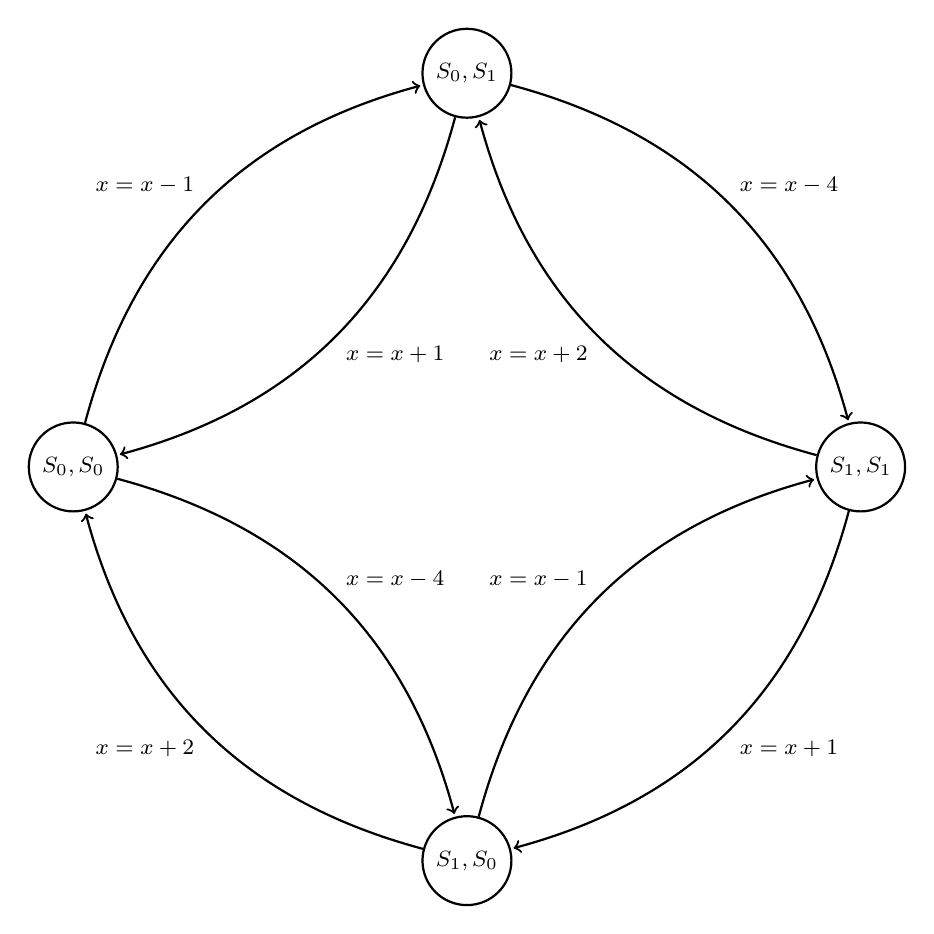
\begin{tikzpicture}[->,shorten >=1pt,auto,node distance=5cm,thick,font=\footnotesize,
    base/.style={circle,draw,minimum size=10pt, text centered}]

    \node[base] (1)
    { $S_0, S_0$ };
    
    \node[base, above of=1, right of=1] (2)
    { $S_0, S_1$ };
    \node[base, below of=2, right of=1] (3)
    { $S_1, S_0$ };
    \node[base, right of=3, above of=3] (4)
    { $S_1, S_1$ };
    
    \path[]
    {
        (1) edge[bend left] node[auto] {$x = x - 1$} (2)
        (2) edge[bend left] node[auto] {$x = x + 1$} (1)
        
        (1) edge[bend left] node[auto] {$x = x - 4$} (3)
        (3) edge[bend left] node[auto] {$x = x + 2$} (1)
        
        (2) edge[bend left] node[auto] {$x = x - 4$} (4)
        (4) edge[bend left] node[auto] {$x = x + 2$} (2)
        
        (3) edge[bend left] node[auto] {$x = x - 1$} (4)
        (4) edge[bend left] node[auto] {$x = x + 1$} (3)
    };
\end{tikzpicture}
\end{center}

\zadatak{c)}

Odrediti ekspandirani asinkroni produkt za prvih 5-10 po volji odabranih članova i nacrtati ga.

\odgovor

Uzmimo $x_0 = 35$.

\begin{center}
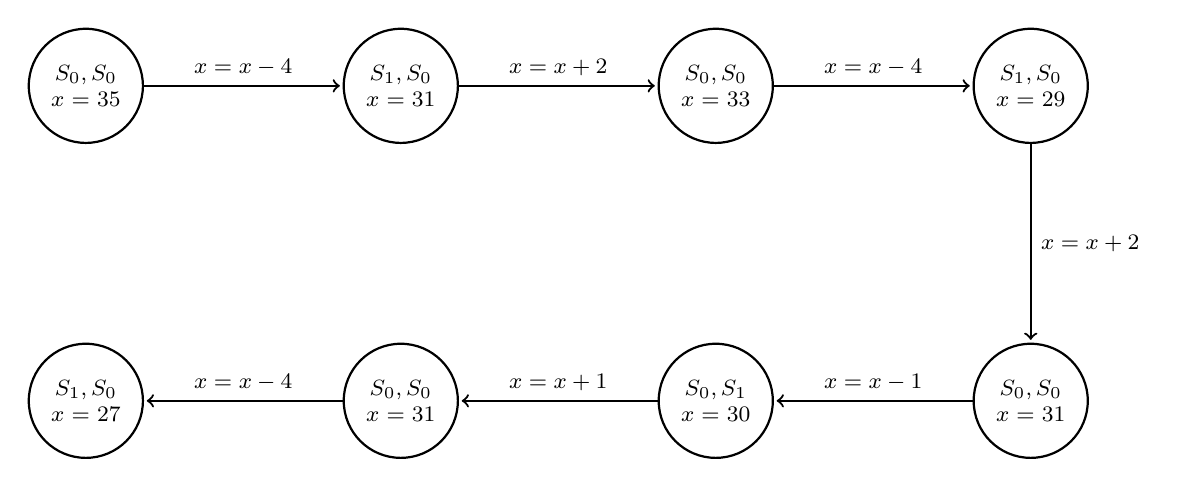
\begin{tikzpicture}[->,shorten >=1pt,auto,node distance=4cm,thick,font=\footnotesize,
    base/.style={circle,draw,minimum size=1cm, text width=1cm, text centered}]

    \node[base] (1)
    {
        $S_0, S_0$
        $x = 35$
    };
    \node[base, right of=1] (2)
    {
        $S_1, S_0$
        $x = 31$
    };
    \node[base, right of=2] (3)
    {
        $S_0, S_0$
        $x = 33$
    };
    \node[base, right of=3] (4)
    {
        $S_1, S_0$
        $x = 29$
    };
    \node[base, below of=4] (5)
    {
        $S_0, S_0$
        $x = 31$
    };
    \node[base, left of=5] (6)
    {
        $S_0, S_1$
        $x = 30$
    };
    
    \node[base, left of=6] (7)
    {
        $S_0, S_0$
        $x = 31$
    };
    
    \node[base, left of=7] (8)
    {
        $S_1, S_0$
        $x = 27$
    };
    
    \path[]
    {
        (1) edge node[above] {$x = x - 4$} (2)
        (2) edge node[above] {$x = x + 2$} (3)
        (3) edge node[above] {$x = x - 4$} (4)
        (4) edge node[right] {$x = x + 2$} (5)
        (5) edge node[above] {$x = x - 1$} (6)
        (6) edge node[above] {$x = x + 1$} (7)
        (7) edge node[above] {$x = x - 4$} (8)
    };
\end{tikzpicture}
\end{center}

\zadatak{d)}

Pomoću ekspandiranog produkta odrediti istinitost LTL formule $\mathbin{\Diamond}\Box p$ ako je $p \equiv x \leq 0$. Obrazložiti rješenje, posebice komentirati mogućnost rješavanja bez primjene programskih alata.

\odgovor

Formula ispituje je li uvijek globalno vrijedi da je $x \leq 0$. Ovo ne vrijedi jer možemo zapeti u petlji $(S_0, S_0) \rightarrow (S_0, S_1) \rightarrow (S_0, S_0)$ za neki $x_0 \geq 1$.

\zadatak{e)}

Pomoću ekspandiranog produkta odrediti istinitost LTL formule $\mathbin{\Diamond} p$ ako je $p \equiv x < 0$. Obrazložiti rješenje, posebice komentirati mogućnost rješavanja bez primjene programskih alata.

\odgovor

Isto kao i iznad - ne vrijedi uvijek $p \equiv x < 0$ jer možemo zapeti u petlji koja će $x$ održavati pozitivnim ako odaberemo pozitivan početni $x$.

\zadatak{f)}

Nacrtati moguću realizaciju Büchi automata za LTL formulu: $\Box(p \wedge q)$.

\odgovor

\begin{center}
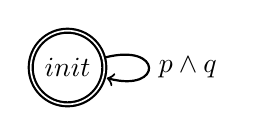
\begin{tikzpicture}[->,shorten >=1pt,auto,node distance=2cm,thick,font=\normal,
    final/.style={double,circle,draw,minimum size=10pt, text centered}]

    \node[final] (1)
    { $init$ };
    
    \path[]
    { (1) edge[loop right] node[auto] {$p \wedge q$} (1) };
\end{tikzpicture}
\end{center}


\pagebreak





\dio{2}

\zadatak{1.}

Instalirajte programski alat \href{http://spinroot.com/spin/Bin/index.html}{Spin}. Instalacija se svodi na kopiranje izvršnog programa. Za one koji hoće više, sve instrukcije jezika \textit{ProMeLa} možete pronaći na \href{http://spinroot.com/spin/Man/promela.html}{ovoj poveznici}, kao i službene upute ("manual") \href{http://spinroot.com/spin/Man/Manual.html}{ovdje}.


\zadatak{2.}

Uredite automate $A_1$ i $A_2$ kao promela procese $A$ i $B$ (vidjeti \hyperref[sec:promela-template]{predložak}). Napomena: Promela datoteku nazvati \texttt{prezime.prm} (npr. \texttt{blaskovic.prm}). Polazeći od zadanog Promela modela koji se sastoji od dva procesa $A$ i $B$ analizirat će se LTL formula $\mathbin{\Diamond}p$ gdje je $p \equiv (x \leq 0)$.


\zadatak{3.}

Pokrenite simulaciju: \texttt{spin -u20 -p -c -g prezime.prm}. Prepišite prvih 12 članova. Pismeno obrazložite istovjetnosti i razlike između ekspandiranog asinkronog produkta iz domaće zadaće i rezultata simulacije.

\odgovor

\begin{ccode}
  1:    proc  0 (A:1) ./src/p-2/prezime.pml:8 (state 1)  [(1)]
  2:    proc  1 (B:1) ./src/p-2/prezime.pml:16 (state 1) [(1)]
  3:    proc  1 (B:1) ./src/p-2/prezime.pml:17 (state 2) [x = (x-1)]
                x = 34
  4:    proc  0 (A:1) ./src/p-2/prezime.pml:9 (state 2)  [x = (x-4)]
                x = 30
  5:    proc  0 (A:1) ./src/p-2/prezime.pml:9 (state 3)  [goto S1]
  6:    proc  1 (B:1) ./src/p-2/prezime.pml:17 (state 3) [goto S1]
  7:    proc  0 (A:1) ./src/p-2/prezime.pml:10 (state 4) [x = (x+2)]
                x = 32
  8:    proc  0 (A:1) ./src/p-2/prezime.pml:10 (state 5) [goto S0]
  9:    proc  1 (B:1) ./src/p-2/prezime.pml:18 (state 4) [x = (x+1)]
                x = 33
 10:    proc  1 (B:1) ./src/p-2/prezime.pml:18 (state 5) [goto S0]
 11:    proc  0 (A:1) ./src/p-2/prezime.pml:9 (state 2)  [x = (x-4)]
                x = 29
 12:    proc  1 (B:1) ./src/p-2/prezime.pml:17 (state 2) [x = (x-1)]
                x = 28
\end{ccode} \newline

\noindent

Ovdje se odvijaju prijelazi u drukčijem redoslijedu (npr. mi smo u prvih 4 iteracija pokretali samo proces 1, ovdje se pokreću naizmjence). Zbog drukčijeg redoslijeda i početne vrijednosti, i konačni rezultat je drukčiji. Jedino što je isto je da će uz dobru vjeru (ako ne bude samo djelovao proces 1) vrijednost konvergirati prema $-\infty$.


\zadatak{4.}

Generirajte analizator: \texttt{spin -a prezime.prm}.


\zadatak{5.}

Prevedite u izvršni oblik npr.: \texttt{gcc -o pan pan.c}


\zadatak{6.}

Pozovite analizator: \texttt{pan -a} ili \texttt{./pan -e}. Pismeno obrazližite je li uvjet $p$ zadovoljen.

\odgovor

Uvjet nije zadovoljen:

\begin{ccode}
assertion violated  !((x<=0)) (at depth 128)
\end{ccode}


\zadatak{7.}

Pokrenite "error trail" opciju (pronalaženje protuprimjera) sa \texttt{spin -t -p -c -g prezime.prm}. Postoji li sekvenca u kojoj varijabla $x$ na kraju poprima vrijednost $x \leq 0$? Koliko koraka (\textit{engl. steps}) sadrži?

\odgovor

Postoji takva sekvenca. Ona sadrži 129 koraka.


\zadatak{8.}

Prepišite instrukcije za Büchi automat koje generira Spin \texttt{spin -f '!<>q'}. Nacrtajte pripadni Büchi automat.

\odgovor

\begin{ccode}
never  {    /* !<>q */
accept_init:
T0_init:
        do
        :: (! ((q))) -> goto T0_init
        od;
}
\end{ccode}

\begin{center}
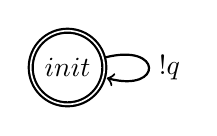
\begin{tikzpicture}[->,shorten >=1pt,auto,node distance=2cm,thick,font=\normal,
    final/.style={draw, circle, double, minimum size=10pt, text centered}]

    \node[final] (1)
    { $init$ };
    
    \path[]
    { (1) edge[loop right] node[auto] {$!q$} (1) };
\end{tikzpicture}
\end{center}


\zadatak{9.}

Prepišite instrukcije za Büchi automat koje generira Spin \texttt{spin -f '![]q'}. Nacrtajte pripadni Büchi automat.

\odgovor

\begin{ccode}
never  {    /* ![]q */
T0_init:
        do
        :: atomic { (! ((q))) -> assert(!(! ((q)))) }
        :: (1) -> goto T0_init
        od;
accept_all:
        skip
}
\end{ccode}

\begin{center}
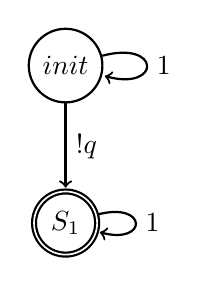
\begin{tikzpicture}[->,shorten >=1pt,auto,node distance=2cm,thick,font=\normal,
    base/.style={draw, circle, minimum size=10pt, text centered},
    final/.style={draw, circle, double, minimum size=10pt, text centered}]

    \node[base] (init)
    { $init$ };
    
    \node[final, below of=init] (1)
    { $S_1$ };
    
    \path[]
    {
        (init) edge[loop right] node[auto] {$1$} (init)
        (init) edge node[auto] {$!q$} (1)
        (1) edge[loop right] node[auto] {$1$} (1)
    };
\end{tikzpicture}
\end{center}


\zadatak{10.}

Na isti način koristeći Spin nacrtajte automat iz Vaše domaće zadaće (pitanje \texttt{f)}).

\odgovor

\begin{ccode}
never  {    /* [](p && q) */
accept_init:
T0_init:
        do
        :: ((p && q)) -> goto T0_init
        od;
}
\end{ccode}

\begin{center}
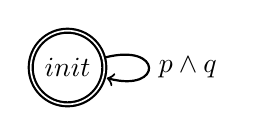
\begin{tikzpicture}[->,shorten >=1pt,auto,node distance=2cm,thick,font=\normal,
    final/.style={draw, circle, double, minimum size=10pt, text centered}]

    \node[final] (1)
    { $init$ };
    
    \path[]
    { (1) edge[loop right] node[auto] {$p \wedge q$} (1) };
\end{tikzpicture}
\end{center}

\pagebreak


\zadatak{11.}

Generirajte analizator sa \texttt{spin -a -o3 prezime.prm}, prevedite te pozovite analizator sa \texttt{pan -d}. Precrtajte tako dobivene FSA. Objasnite razlike kao i istovjetnosti prema automatima iz domaće zadaće. Usporedite stanja prema slici automata i stanja dobivena s opcijom \texttt{pan -d}. U čemu je razlika?

\odgovor

\begin{center}
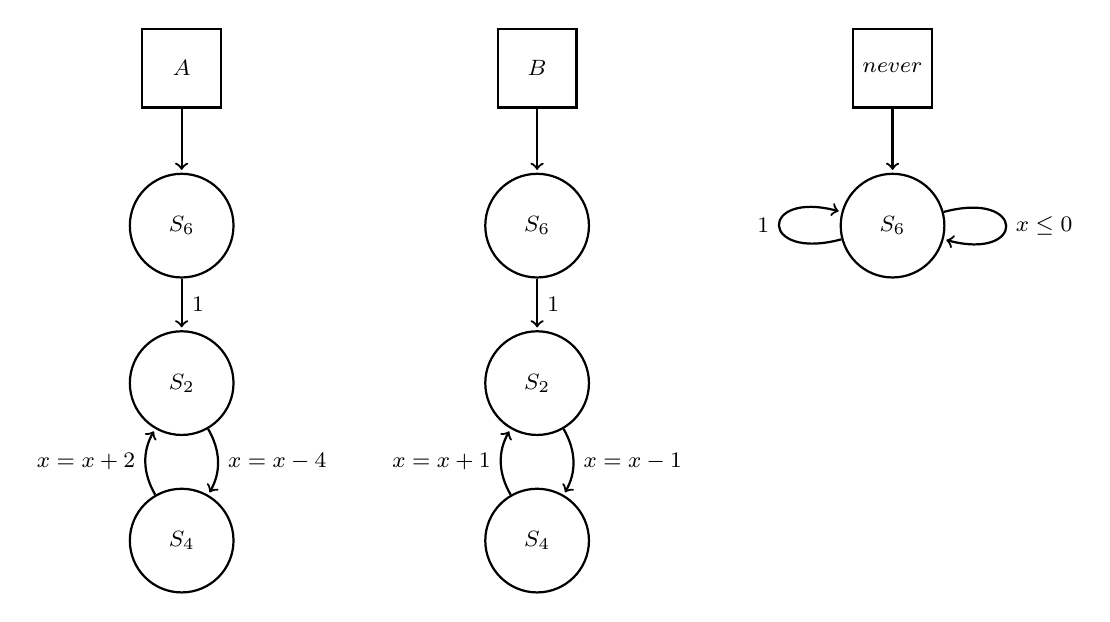
\begin{tikzpicture}[->,shorten >=1pt,auto,node distance=2cm,thick,font=\footnotesize,
    proc/.style={draw, rectangle, minimum size=1cm, text centered},
    base/.style={draw, circle ,minimum size=1cm, text width=1cm, text centered}]

    \node[proc] (A)
    { $A$ };
    
    \node[base, below of=A] (S6A)
    { $S_6$ };
    
    \node[base, below of=S6A] (S2A)
    { $S_2$ };
    
    \node[base, below of=S2A] (S4A)
    { $S_4$ };
    
    %------------------------------------------------

    \node[proc, right of=A] (B) [right=2cm]
    { $B$ };
    
    \node[base, below of=B] (S6B)
    { $S_6$ };
    
    \node[base, below of=S6B] (S2B)
    { $S_2$ };
    
    \node[base, below of=S2B] (S4B)
    { $S_4$ };
    
    %------------------------------------------------
    
    \node[proc, right of=B] (never) [right=2cm]
    { $never$  };
    
    \node[base, below of=never] (S6never)
    { $S_6$ };
    
    \path[]
    {
        (A) edge node[auto] {} (S6A)
        (S6A) edge node[auto] {1} (S2A)
        (S2A) edge[bend left] node[auto] {$x = x - 4$} (S4A)
        (S4A) edge[bend left] node[auto] {$x = x + 2$} (S2A)
        
        (B) edge node[auto] {} (S6B)
        (S6B) edge node[auto] {1} (S2B)
        (S2B) edge[bend left] node[auto] {$x = x - 1$} (S4B)
        (S4B) edge[bend left] node[auto] {$x = x + 1$} (S2B)
        
        (never) edge node[auto] {} (S6never)
        (S6never) edge[loop left] node[auto] {1} (S6never)
        (S6never) edge[loop right] node[auto] {$x \leq 0$} (S6never)
    };
\end{tikzpicture}
\end{center} \newline

\noindent
Prijelazi su isti. Međutim, naredba nam je izbacila i automat za \texttt{never}.

\pagebreak



\dio{3}

Ponovite postupak za $\mathbin{\Diamond}\Box p$ (modificirati "\textit{never claim}" \texttt{spin -f "<>[]p"} na kraju prezime.prm datoteke).

\zadatak{1.}

Postoji li sekvenca u kojoj varijabla $x$ na kraju poprima vrijednost $x \leq 0$?

\odgovor

Pokretanjem \texttt{spin -a prezime.prm} utvrđujemo da takva sekvenca postoji.

\zadatak{2.}

Koliko koraka (\textit{engl. steps}) sadrži?

\odgovor

Zadnjih par linija ispisa \texttt{spin -t -p -c -g ./src/p-3/prezime.pml} nam vraća:

\begin{ccode}
136:    proc  0 (A:1) prezime.pml:9 (state 2)    [x = (x-4)]
                x = -2
Never claim moves to line 25    [((x<=0))]
138:    proc  1 (B:1) prezime.pml:18 (state 4)   [x = (x+1)]
                x = -1
  <<<<<START OF CYCLE>>>>>
Never claim moves to line 30    [((x<=0))]
140:    proc  1 (B:1) prezime.pml:17 (state 2)   [x = (x-1)]
                x = -2
142:    proc  1 (B:1) prezime.pml:18 (state 4)   [x = (x+1)]
                x = -1
spin: trail ends after 142 steps
\end{ccode} \newline

\noindent
Stoga utvrđujemo da se to događa nakon 139 koraka.

\zadatak{3.}

Je li moguće problem riješiti bez LTL formule, samo pomoću \texttt{assert naredbi}? Obrazložite odgovor.

\odgovor

To nije moguće. Razlog za to je što kad bi koristili \texttt{assert}, moramo ga koristiti nakon što je uvjet ispunjen. Ako znamo kad je uvjet ispunjen, koja je svrha validacije?

\zadatak{4.}

Je li moguće problem riješiti bez LTL formule, samo pomoću simulacije? Obrazložite odgovor.

\odgovor

To isto nije moguće. Imamo beskonačno puteva izvođenja, i još k tome petlju!

\pagebreak





\dio{4}

Zadan je Promela model komunikacijskog protokola koji opisuje dio moguće realizacije protokola za preuzimanje datoteka (\textit{engl. download}):

\begin{ccode}
mtype = { ini, ack, dreq, data, shutup, quiet, dead };
chan M = [N] of { mtype };
chan W = [N] of { mtype };

active proctype Mproc() {
    W!ini;
    M?ack;
    
    timeout ->
        if
            :: W!shutup
            :: W!dreq;
                M?data ->
                    do
                        :: W!data
                        :: W!shutup;
                        break
                    od
        fi;

    M?shutup;
    W!quiet;
    M?dead
}
active proctype Wproc() {
    W?ini;
    M!ack;
    
    do
        :: W?dreq ->
            M!data
        :: W?data ->
            #if 1
            M!data
            #else
            skip
            #endif
        :: W?shutup ->
            M!shutup;
        break
    od;
    
    W?quiet;
    M!dead
}
\end{ccode} \newline

\noindent
Ako je $N = 16$, pomoću programskog alata \texttt{Spin} odredite:

\zadatak{a)}

Iz kojih stanja nema napretka (nastupa tzv. potpuni zastoj, \textit{engl. deadlock})?

\odgovor

Prvo moramo skicirati automate:

\begin{center}
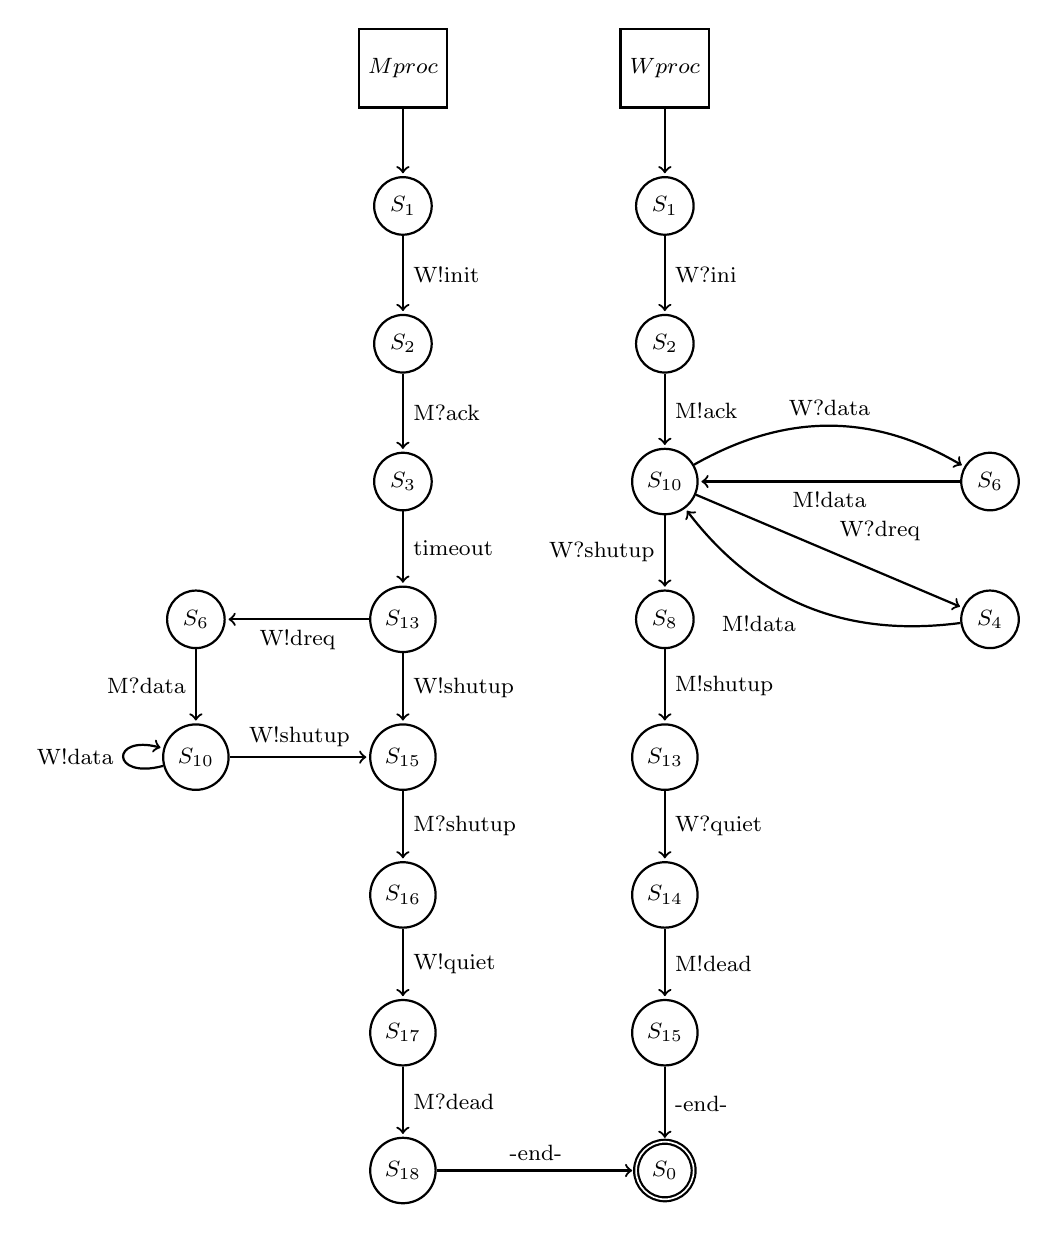
\begin{tikzpicture}[->, shorten >=1pt, auto, node distance=1.75cm, thick, font=\footnotesize,
    proc/.style={draw, rectangle, minimum size=1cm, text centered},
    base/.style={draw, circle, minimum size=0.5cm, text centered},
    final/.style={draw, circle, double, minimum size=0.5cm, text centered}]

    \node[proc] (Mproc)
    { $Mproc$ };
    
    \node[base, below of=Mproc] (S1A)
    { $S_1$ };
    
    \node[base, below of=S1A] (S2A)
    { $S_2$ };
    
    \node[base, below of=S2A] (S3A)
    { $S_3$ };
    
    \node[base, below of=S3A] (S13A)
    { $S_{13}$ };


    \node[base, left of=S13A] (S6A) [left=0.5cm]
    { $S_6$ };
    
    \node[base, below of=S6A] (S10A)
    { $S_{10}$ };
    
    \node[base, below of=S13A] (S15A)
    { $S_{15}$ };
    
    
    \node[base, below of=S15A] (S16A)
    { $S_{16}$ };
    
    \node[base, below of=S16A] (S17A)
    { $S_{17}$ };
    
    \node[base, below of=S17A] (S18A)
    { $S_{18}$ };
    
    % ---------------------------------------------------------
    
    \node[proc, right of=Mproc] (Wproc) [right=1cm]
    { $Wproc$ };
    
    \node[base, below of=Wproc] (S1B)
    { $S_1$ };
    
    \node[base, below of=S1B] (S2B)
    { $S_2$ };
    
    \node[base, below of=S2B] (S10B)
    { $S_{10}$ };


    \node[base, below of=S10B] (S8B)
    { $S_8$ };
    
    \node[base, below of=S8B] (S13B)
    { $S_{13}$ };
    
    \node[base, below of=S13B] (S14B)
    { $S_{14}$ };
    
    \node[base, below of=S14B] (S15B)
    { $S_{15}$ };
    
    \node[final, below of=S15B] (S0)
    { $S_0$ };

    
    \node[base, right of=S10B] (S6B) [right=2cm]
    { $S_6$ };
    
    \node[base, below of=S6B] (S4B)
    { $S_4$ };
    
    \path[]
    {
        (Mproc) edge node[auto] {} (S1A)
        (S1A) edge node[auto] {W!init} (S2A)
        (S2A) edge node[auto] {M?ack} (S3A)
        (S3A) edge node[auto] {timeout} (S13A)
        
        (S13A) edge node[auto] {W!dreq} (S6A)
        (S6A) edge node[left] {M?data} (S10A)
        (S10A) edge[loop left] node[auto] {W!data} (S10A)
        (S10A) edge node[auto] {W!shutup} (S15A)
        
        (S13A) edge node[auto] {W!shutup} (S15A)
        
        (S15A) edge node[auto] {M?shutup} (S16A)
        (S16A) edge node[auto] {W!quiet} (S17A)
        (S17A) edge node[auto] {M?dead} (S18A)
        
        (S18A) edge node[auto] {-end-} (S0)
        
        % --------------------------------------------------
        
        (Wproc) edge node[auto] {} (S1B)
        (S1B) edge node[auto] {W?ini} (S2B)
        (S2B) edge node[auto] {M!ack} (S10B)
        
        (S10B) edge node[left] {W?shutup} (S8B)
        (S8B) edge node[auto] {M!shutup} (S13B)
        (S13B) edge node[auto] {W?quiet} (S14B)
        (S14B) edge node[auto] {M!dead} (S15B)
        
        (S15B) edge node[auto] {-end-} (S0)
        
        (S10B) edge[bend left] node[auto] {W?data} (S6B)
        (S6B) edge node[auto] {M!data} (S10B)
        
        (S10B) edge node[auto] {W?dreq} (S4B)
        (S4B) edge[bend left] node[auto] {M!data} (S10B)
    };
\end{tikzpicture}
\end{center} \newline

\noindent
Kao što vidimo sa slike, potpuni zastoj može nastupiti u $S_{10}$.


\zadatak{b)}

Dolazi li protokol u završno stanje?

\odgovor

Da. Ovo možemo provjeriti s \texttt{spin -p -c -g ./src/p-4/prezime.pml}. Zadnjih par linija ispisa nam daju:

\begin{ccode}
 12:    proc  0 (Mproc:1) prezime.pml:24 (state 15)      [M?shutup]
                queue 2 (M):
                queue 1 (W):
  1   W!quiet
 13:    proc  0 (Mproc:1) prezime.pml:25 (state 16)      [W!quiet]
                queue 2 (M):
                queue 1 (W): [quiet]
  1   .   W?quiet
 14:    proc  1 (Wproc:1) prezime.pml:47 (state 13)      [W?quiet]
                queue 2 (M):
                queue 1 (W):
  2   .   M!dead
 15:    proc  1 (Wproc:1) prezime.pml:48 (state 14)      [M!dead]
                queue 2 (M): [dead]
                queue 1 (W):
  2   M?dead
 16:    proc  0 (Mproc:1) prezime.pml:26 (state 17)      [M?dead]
                queue 2 (M):
                queue 1 (W):
 16:    proc  1 (Wproc:1)           terminates
 16:    proc  0 (Mproc:1)       terminates
\end{ccode} \newline

\noindent
Ovo znači da je moguće doći do konačnog stanja.


\pagebreak

\sekcija{Dodatak A - ProMeLa predložak}
\label{sec:promela-template}

\newline \newline

\begin{ccode}
#define N 35
#define p (x <= 0)

int x = N;

active proctype A() {
do
    ...
od;
}

active proctype B() {
do
    ...
od;
}

never { /* LTL formula */
    ...
}

\end{ccode}

\end{document}